\documentclass{article}
\usepackage{blindtext}
\usepackage[utf8]{inputenc}
\usepackage{amsmath,bm}
\usepackage{amstext}
\usepackage{amsfonts}
\usepackage{amsmath}
\usepackage{multirow}
\usepackage{enumerate}
\usepackage{xeCJK}
\setCJKmainfont{STKaiti}
\usepackage[noend]{algpseudocode}
\usepackage{algorithmicx,algorithm}
 \usepackage{graphicx}
 \usepackage{float}
\usepackage{listings}
\lstset{
	columns=fixed,       
	numbers=left,                                        % 在左侧显示行号
	numberstyle=\tiny\color{gray},                       % 设定行号格式
	frame=none,                                          % 不显示背景边框
	keywordstyle=\color[RGB]{40,40,255},                 % 设定关键字颜色
	numberstyle=\footnotesize\color{darkgray},           
	commentstyle=\it\color[RGB]{0,96,96},                % 设置代码注释的格式
	stringstyle=\rmfamily\slshape\color[RGB]{128,0,0},   % 设置字符串格式
	showstringspaces=false,                              % 不显示字符串中的空格
	language=matlab,                                        % 设置语言
}

\title{矩阵论及其应用实习题}
\author{陈轶洲 MF20330010}
\begin{document}
	\maketitle
	\numberwithin{equation}{section}
	
\section{实验环境}

计算机型号:MacBook Air (13-inch, Early 2015)\\
操作系统:Mac os\\
编程语言:Matlab
	
	
\section{CPU时间}
输入第一组数据:
\begin{figure}[h]
	\centering
	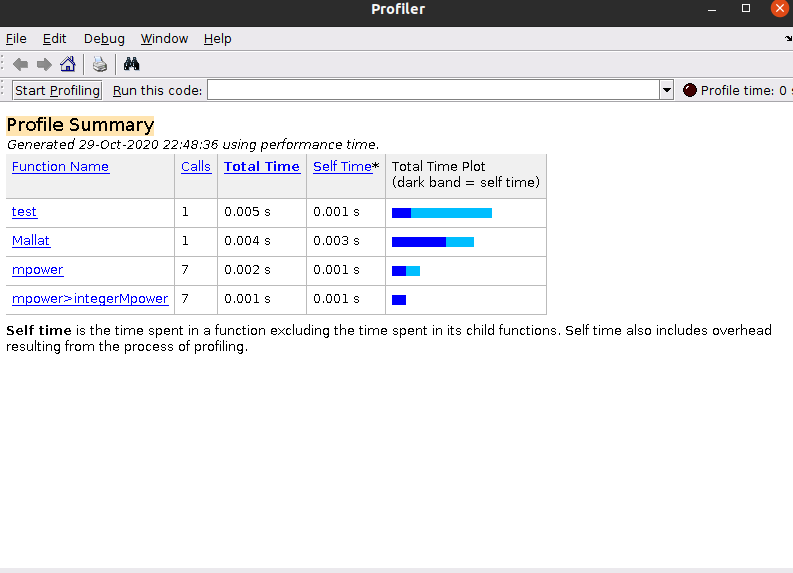
\includegraphics[scale=0.6]{test1.png}
\end{figure}

输入第二组数据:
\begin{figure}[h]
	\centering
	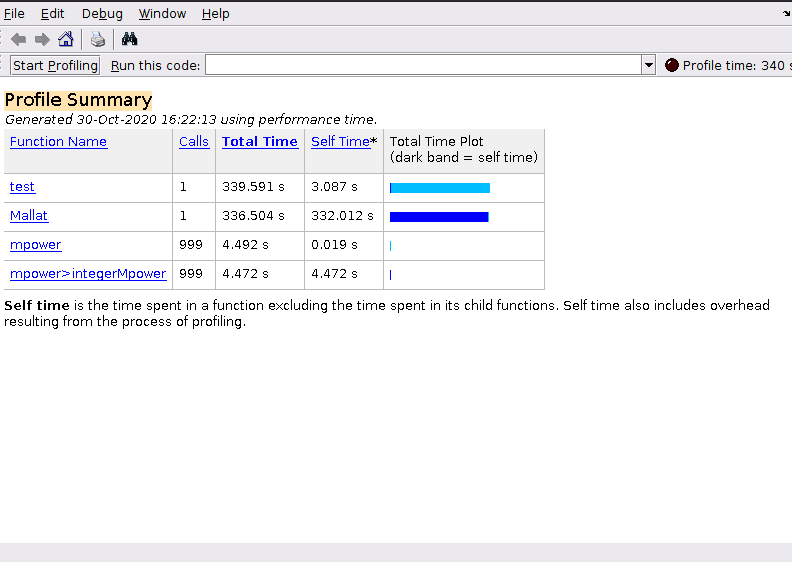
\includegraphics[scale=0.6]{test2.png}
\end{figure}

\section{算法说明}
\subsection{算法步骤}
	\begin{algorithm}[H]
		\caption{正交匹配追踪算法} 
		\hspace*{0.02in} {\bf Input:} 
		观测数据向量$ y\in R^{M\times 1},$ 字典矩阵 $ A \in R^{M\times N},$ 稀疏性指标 $K\in N$\\
		\hspace*{0.02in} {\bf Output:} 
		稀疏的信号向量$ x \in R^{N\times 1}$ 
		\begin{algorithmic}[1]
			\State 初始化:$ \Omega_0=\phi,r_0=y,k=1 $ 
			\While{$ k\leq K $} 
			\State $ j_k\in \arg{\max_j{|(r_{k-1},a_j)|}} $
			\State $ \Omega_k = \Omega_{k-1}\cup \{j_k\} $
			\State $ x_k = (A_{\Omega_k}^{T}A_{\Omega_k})^{-1}A_{\Omega_k}^{T}y $
			\State $ r_k = y-A_{\Omega_k}x_k $
			\State $ k += 1 $
			\EndWhile
			\State $  \hat{x}(i) = \left\{
			\begin{aligned}
				x_K(i) \qquad i\in \Omega_K\\
				0 \qquad others
			\end{aligned} 
			\right. $
			\State \Return $ \hat{x} $
		\end{algorithmic}
	\end{algorithm}
\subsection{变量说明}
使用Matlab设计的正交匹配追踪算法中,对变量做如下定义:\\
1.A为测度矩阵,规模为$ M\times N $;\\
2.y为观测所得向量,规模为$ M\times 1 $;\\
3.K为稀疏性指标,为正整数;\\
4.x为待还原向量,规模为$ N\times 1 $;\\
5.r为残差向量,规模为$ M\times 1 $;\\
6.At,每轮迭代时被选中的列\\
7.$ x_l $为最小二乘解

\subsection{程序清单}
首先在Mallat.m中实现正交匹配追踪算法:
\begin{lstlisting}
function [ x ] = Mallat(y,A,K)
	[M,N] = size(A);%字典矩阵的规模
	x = zeros(N, 1);%需要重构的解向量x
	At = zeros(M, K);%存储每轮迭代时A中被选中的列
	x_pos = zeros(1, K);%存储每轮迭代时A中被选中列的序号
	r = y;%残差向量,初始化为y
	
	for ii = 1:K%迭代K轮
		product = A'*r;%计算矩阵各列与残差的点积
		[val, pos] = max(abs(product));%找到与残差最相关的列
		At(:,ii) = A(:,pos);%将被选中的列存储到At中
		x_pos(ii) = pos;%记录被选中列的序号
		A(:,pos) = zeros(M,1);%清零A的这一列,其实此行可以不要,因为它与残差正交
		x_l = (At(:,1:ii)'*At(:,1:ii))^(-1)*At(:,1:ii)'*y;%最小二乘解
		r = y - At(:,1:ii)*x_l;%更新残差
	end
	
	x(x_pos) = x_l;
end
\end{lstlisting}
接着在test.m中对两组规模的数据进行测试
\begin{lstlisting}
	K=8;
	M=50;
	N=100;
	A=randn(M,N);
	y=randn(M,1);
	x1 = Mallat(y,A,K);
	
	K=1000;
	M=15000;
	N=23000;
	A=randn(M,N);
	y=randn(M,1);
	x2 = Mallat(y,A,K);
\end{lstlisting}

\section{运行结果及分析}
第一组数据的解向量:
\begin{figure}[h]
	\centering
	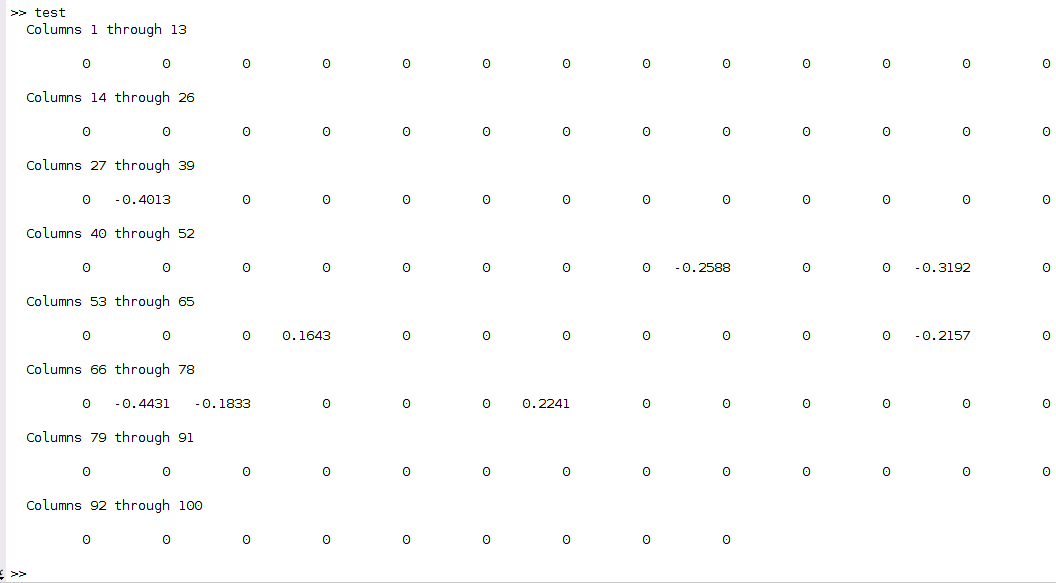
\includegraphics[scale=0.6]{output.png}
\end{figure}

从结果可以看出,使用正交匹配追踪算法可以有效恢复信号,并通过稀疏性指标控制向量的稀疏性
\section{实验总结}
通过本次实验,让我对信号处理有了初步的了解,其中所涉及的矩阵论知识也强化了我对矩阵的特性以及矩阵运算有了进一步的认识。

\end{document}
